\documentclass[12pt,a4paper]{article}

% Essential packages first
\usepackage{amsthm,amssymb,amsmath}
\usepackage[a4paper, top=40mm, bottom=40mm, outer=25mm, inner=35mm]{geometry}
\usepackage[final]{graphicx}
\graphicspath{{./img/}}

% Table and formatting packages
\usepackage{booktabs}
\usepackage{longtable}
\usepackage{array}
\usepackage{multirow}
\usepackage{multicol}
\usepackage{tabulary}
\usepackage{tabularx}
\usepackage{rotating}

% Figure and caption packages
\usepackage{float}
\usepackage[export]{adjustbox}
\usepackage{subfig}
\usepackage{caption}

% Colors and hyperlinks
\usepackage[usenames,dvipsnames,svgnames,table]{xcolor}
\usepackage{hyperref}

% Page layout and headers
\usepackage{fancyhdr}
\usepackage{lastpage}
\usepackage{etoolbox}

% Table of contents customization
\usepackage{tocloft}
\usepackage[nottoc]{tocbibind}

% Algorithm packages
\usepackage{algorithm}
\usepackage{algorithmic}

% Code listing packages
\usepackage[final]{listings}

% Other useful packages
\usepackage{framed}
\usepackage{indentfirst}
\usepackage{setspace}
\usepackage{morewrites}

% Persian language support - must be loaded last
\usepackage[extrafootnotefeatures, localise=on, numerals=latin]{xepersian}

% Font configuration - simplified to avoid font file issues
\settextfont{XB Niloofar}
\setlatintextfont{Times New Roman}
\setdigitfont{XB Niloofar}

% Define colors for hyperlinks
\hypersetup{
    colorlinks=true,
    linkcolor=black,
    filecolor=magenta,      
    urlcolor=cyan,
    citecolor=black,
    unicode=true
}

% Custom commands for document information
\newcommand{\universitytitle}{دانشگاه تهران}
\newcommand{\facultytitle}{دانشکده مهندسی برق و کامپیوتر}
\newcommand{\coursetitle}{درس شبکه‌های عصبی و یادگیری عمیق}
\newcommand{\assignmenttitle}{پاسخ تمرین شماره یک}
\newcommand{\assignmentnumber}{۱} % Modified this

% Title page header
\newcommand{\makeheader}{
    \noindent
    \makebox[\textwidth][c]{%
        \begin{minipage}[t]{0.15\textwidth}
            
\includegraphics[height=2.5cm]{logo1.png} % uniform height
        \end{minipage}%
        \hfill
        \begin{minipage}[t]{0.7\textwidth}
            \centering
            \Large
            \universitytitle\\[0.3em]
            \facultytitle
        \end{minipage}%
        \hfill
        \begin{minipage}[t]{0.15\textwidth}
            
\includegraphics[height=2.5cm]{logo2.png} % same height
        \end{minipage}%
    }
    \vspace{1em} % optional spacing after header
}

% Student information table
\newcommand{\studenttable}[4]{
    \begin{table}[h]
        \centering
        \begin{tabular}{|p{3cm}|p{5cm}|p{4cm}|}
            \hline
            \textbf{سوال یک:} & \textbf{نام و نام خانوادگی} & \textbf{شماره دانشجویی} \\
            \hline
            سوال دو: & #1 & #2 \\
            \hline
            & #3 & #4 \\
            \hline
        \end{tabular}
    \end{table}
}

% Custom section numbering for Persian
\renewcommand{\thesection}{\arabic{section}}
\renewcommand{\thesubsection}{\arabic{section}--\arabic{subsection}}
\renewcommand{\thesubsubsection}{\arabic{section}--\arabic{subsection}--\arabic{subsubsection}}

% Table and figure caption formatting
\captionsetup[table]{name=جدول}
\captionsetup[figure]{name=شکل}

% Set numbering depth
\setcounter{secnumdepth}{3}
\setcounter{tocdepth}{3}

% Line spacing
\doublespacing
% For the first page of each section, also show the header




% Define algorithm translations
\renewcommand{\algorithmicrequire}{\textbf{ورودی:}}
\renewcommand{\algorithmicensure}{\textbf{خروجی:}}
\renewcommand{\algorithmicend}{\textbf{پایان}}
\renewcommand{\algorithmicif}{\textbf{اگر}}
\renewcommand{\algorithmicthen}{\textbf{آنگاه}}
\renewcommand{\algorithmicelse}{\textbf{وگرنه}}
\renewcommand{\algorithmicfor}{\textbf{برای}}
\renewcommand{\algorithmicdo}{\textbf{انجام بده}}
\renewcommand{\algorithmicwhile}{\textbf{تا زمانی که}}
\renewcommand{\algorithmicreturn}{\textbf{بازگردان}}

% Code listing style
\lstdefinestyle{myStyle}{
    basicstyle=\ttfamily,
    keywordstyle=\color{blue}\bfseries,
    commentstyle=\color{LimeGreen},
    stringstyle=\ttfamily\color{red},
    showstringspaces=false,
    breaklines=true,
    breakatwhitespace=false,
    numbers=right,
    numberstyle=\footnotesize\lr,
    numbersep=-10pt,
    frame=single,
    captionpos=b,
    captiondirection=RTL
}
\lstset{style=myStyle}

% List names in Persian
\def\lstlistingname{\rl{برنامهٔ}}
\def\lstlistlistingname{\rl{فهرست برنامه‌ها}}
\def\listalgorithmname{فهرست الگوریتم‌ها}
\def\listfigurename{فهرست تصویرها}
\def\listtablename{فهرست جدول‌ها}

% Theorem environments
\theoremstyle{definition}
\newtheorem{definition}{تعریف}[section]
\newtheorem{theorem}[definition]{قضیه}
\newtheorem{lemma}[definition]{لم}
\newtheorem{proposition}[definition]{گزاره}
\newtheorem{corollary}[definition]{نتیجه}
\newtheorem{remark}[definition]{ملاحظه}
\newtheorem{example}[definition]{مثال}

% Rename proof
\renewcommand\proofname{\textbf{برهان}}

% Bibliography name
\renewcommand{\refname}{مراجع}

% Document starts here
\begin{document}

% Right-to-left text direction for Persian
\setRTL

% Header
\makeheader
\vspace{1cm}

% Course and assignment title
\begin{center}
    % خط بالایی
    \rule{\textwidth}{0.4pt} \\[0.5em]

    % متن اصلی
    \textbf{{\Large درس شبکه‌های عصبی و یادگیری عمیق} \\[0.5em]
    {\Large پاسخ تمرین شماره یک \underline{(اصلاح شود)}} \\[0.5em]}
 % خط کشیده برای اصلاح شود
    % خط پایینی
    \rule{\textwidth}{0.4pt}
\end{center}


\vspace{1cm}

\begin{center} % this centers everything
    {\large دانشجویان:} \\[0.5em] % title

    % Student information table without black lines
    \begin{tabular}{c c c} % two columns, centered
        سوال یک: & نام و نام خانوادگی  & شماره دانشجویی \\
        سوال دو: & نام و نام خانوداگی  & شماره دانشجویی \\
        % اضافه کردن سطرهای دیگر در صورت نیاز
    \end{tabular}
\end{center}
\vspace{1cm}

% Table of contents
\newpage
\tableofcontents

\newpage

% List of figures
\listoffigures
\vspace{1cm}
\newpage

% List of tables
\listoftables
\newpage

\pagestyle{fancy}
\fancyhf{} % Clear all header and footer fields
\fancyhead[R]{\ifnum\value{section}>0 \thesection\ \leftmark\fi} % Right header with section number and name
\renewcommand{\headrulewidth}{0.4pt} % Line thickness under header
\renewcommand{\sectionmark}[1]{\markboth{#1}{}} % Define what goes into \leftmark
\section{\textbf{عنوان سوال}}

در این بخش، سؤال اصلی مطرح می‌شود و نکات مهم مرتبط با آن شرح داده می‌شوند. دانشجو باید با توجه به دستورالعمل‌ها و توضیحات ارائه‌شده، پاسخ مناسب را ارائه کند. این قسمت شامل مقدمه‌ای کوتاه درباره موضوع، محدودیت‌ها، و اهداف مورد انتظار است تا چارچوب حل سؤال مشخص شود.


\subsection{عنوان زیر بخش}

متن سوال اول در اینجا نوشته می‌شود. این بخش شامل توضیحات، تحلیل‌ها و پاسخ‌های مربوط به سوال اول است. می‌توانید از فرمول‌های ریاضی مانند $y = f(x)$ و همچنین معادلات پیچیده‌تر استفاده کنید:


% Sample table
\begin{table}[h]
    \centering
    \caption{پارامترهای مدل}
    \label{tab:hyperparameters}
    \begin{tabular}{|c|c|}
        \hline
        \textbf{پارامتر} & \textbf{مقدار} \\
        \hline
        اندازه دسته (\lr{Batch Size}) & 64 \\
        \hline
        نسبت آموزش، اعتبارسنجی، تست & 70\% - 15\% - 15\% \\
        \hline
        بهینه‌ساز & \lr{Adam} \\
        \hline
        نرخ یادگیری & $0.001$ \\
        \hline
        تابع هزینه & \lr{MSE} \\
        \hline
    \end{tabular}
\end{table}


\subsection{عنوان زیر بخش دوم}

\subsubsection{عنوان زیر بخش زیر بخش}

نتایج تجربی و تحلیل آن‌ها در این بخش ارائه می‌شود. می‌توانید از شکل‌ها و نمودارها استفاده کنید:

% Sample figure placeholder (remove if no image available)
\begin{figure}[H]
    \centering
    % Comment out the includegraphics line if image doesn't exist
    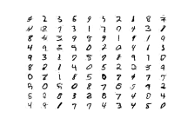
\includegraphics[width=0.6\textwidth]{Picture1.png}
    \caption{مجموعه‌داده MNIST}
    \label{fig:results}
\end{figure}

\subsubsection{عنوان زیربخش زیر بخش}

تفسیر دقیق نتایج و مقایسه با سایر روش‌ها در این قسمت ارائه می‌شود.

% Add more sections as needed for additional questions

\newpage

\section{\textbf{عنوان سوال دوم}}

در این بخش، سؤال اصلی مطرح می‌شود و نکات مهم مرتبط با آن شرح داده می‌شوند. دانشجو باید با توجه به دستورالعمل‌ها و توضیحات ارائه‌شده، پاسخ مناسب را ارائه کند. این قسمت شامل مقدمه‌ای کوتاه درباره موضوع، محدودیت‌ها، و اهداف مورد انتظار است تا چارچوب حل سؤال مشخص شود.


\end{document}